%       10        20        30        40        50        60       70        80        90        100
%234567890123456789012345678901234567890123456789012345678901234567890123456789012345678901234567890

\documentclass{article}
\usepackage[utf8]{inputenc}

%%%%%%%%%%%%%%%%%%%%%%%%%%%%%%%%%%%%%% LOAD AMS LaTeX Packages %%%%%%%%%%%%%%%%%%%%%%%%%%%%%%%%%%%%%

\usepackage{amsmath}
\usepackage{amssymb}
\usepackage{amsfonts}
\usepackage{graphicx}
\usepackage{float}
% As per the LaTeX Wiki book dvips knows a wider range of colors than xcolor alone (try 'svgnames')

\usepackage[dvipsnames]{xcolor}

% package to allow colored source code listings

\usepackage{listings}

\usepackage{fancyhdr}
\usepackage{enumitem}
\pagestyle{fancy}
\fancyhead{}

\fancyhead[L]{\textbf{NAME: Randy Li}} % TYPE YOUR NAME HERE!
\fancyhead[C]{\textbf{CA 01}}              % TYPE THE ASSGNMENT NAME HERE!
\fancyhead[R]{\textbf{SID: 917196816}}     % TYPE YOUR STUDENT ID HERE!

\fancyfoot[L]{CRN 38665}
\fancyfoot[C]{--~\thepage~--}
\fancyfoot[R]{\today}

% Create a language setting for LaTeX
% One can change the language for each code-block optionally
% \lstset
% {
%     language=[LaTeX]TeX,
%     breaklines=true,
%     basicstyle=\tt\scriptsize,
%     keywordstyle=\color{blue},
%     identifierstyle=\color{magenta},
% }

% I like space between paragraphs, since it makes the document more readable. However, this does not
% seem to change the spacing between paragraphs contained in an item of a list.

\setlength{\parskip}{03pt} % default: \parskip = 12  pt

%%%%%%%%%%%%%%%%%%%%%%%%%%%%%%%%%%%%% EGP's LOCAL LaTeX MACROS %%%%%%%%%%%%%%%%%%%%%%%%%%%%%%%%%%%%%

\newcommand{\bs}[1]{\boldsymbol{#1}}


%%%%%%%%%%%%%%%%%%%%%%%%%%%%%%%%%%%%%% TITLE, AUTHOR AND DATE %%%%%%%%%%%%%%%%%%%%%%%%%%%%%%%%%%%%%%
\title{MAT 167 WQ 2022 CA 01 Report}
\author{Randy Li} %YOUR NAME
\date{February 4, 2024}
%\date{January 2022}



\begin{document}

\maketitle
\tableofcontents
\newpage

\section{Introduction and Motivation}
Linear Algebra can be used widely in our real applications, such as machine learning and pattern recognition, data mining and search engine, and signal and image processing. All these application use matrix transformation to process the data. This report will explore specifically about signal processing. Signal processing is a the process of converting the compression or encoded audio into the form closer to the original. In this project, we will do signal processing by compressing each signal matrix to differnt extents and accomplish that by using matlab. 

\section{Data Set}

The data set for signal processing is a matrix file called \texttt{CA\_01.mat}, which is file downloaded from canvas.\\
Since, we have load the matrix, x will be the signal matrix data we used. U will be the orthonormal matrix of the original matrix. \\


\section{Procedure}

\subsection{Loading and Understanding the Data}
Part a)\\
Step1: Use "load \texttt{CA\_01.mat}" to load the matrix to the project.\\
Step2: Draw the signal x\\
Here is the original figure:\\
\begin{figure}[H]
  \centering
  \includegraphics[width=0.8\textwidth]{Fig_01.png}
  \label{fig_01}
\end{figure}
\subsection{Finding Orthonormal Basis Vectors}
b) Find the orthonormal basis vectors by using the Discrete Cosine Transform formula:\\
\begin{equation}
    f_k(x) = \cos\left(\frac{k\pi(x - 1)}{7}\right), \quad k \in \{0, 1, 2, 3, 4, 5, 6, 7\}
\end{equation}\\
Step2: Create a matrix A of orthonormal basis vectors by using the following code:\\
\begin{verbatim}
    A=[A arrayfun(@(x) cos(k*pi*(x-1)/7), [1:8]')];
\end{verbatim}
Each column vectors will be:\\
\begin{equation}
    \begin{bmatrix}
        \cos\left(\frac{2\pi(1-1)}{7}\right) \\
        \cos\left(\frac{2\pi(2-1)}{7}\right) \\
        \cos\left(\frac{2\pi(3-1)}{7}\right) \\
        \cos\left(\frac{2\pi(4-1)}{7}\right) \\
        \cos\left(\frac{2\pi(5-1)}{7}\right) \\
        \cos\left(\frac{2\pi(6-1)}{7}\right) \\
        \cos\left(\frac{2\pi(7-1)}{7}\right) \\
        \cos\left(\frac{2\pi(8-1)}{7}\right) \\
    \end{bmatrix}
\end{equation}
Here is the Matrix A:\\
\begin{verbatim}
A=
    1.0000    1.0000    1.0000    1.0000    1.0000    1.0000    1.0000    1.0000
    1.0000    0.9010    0.6235    0.2225   -0.2225   -0.6235   -0.9010   -1.0000
    1.0000    0.6235   -0.2225   -0.9010   -0.9010   -0.2225    0.6235    1.0000
    1.0000    0.2225   -0.9010   -0.6235    0.6235    0.9010   -0.2225   -1.0000
    1.0000   -0.2225   -0.9010    0.6235    0.6235   -0.9010   -0.2225    1.0000
    1.0000   -0.6235   -0.2225    0.9010   -0.9010    0.2225    0.6235   -1.0000
    1.0000   -0.9010    0.6235   -0.2225   -0.2225    0.6235   -0.9010    1.0000
    1.0000   -1.0000    1.0000   -1.0000    1.0000   -1.0000    1.0000   -1.0000
\end{verbatim}

Step 3: Determine whether A is orthonormal or not by using the formula $A^TA$.\\
Here is the result of $A^TA$:\\
\begin{verbatim}
A^TA =8.0000         0    1.0000    0.0000    1.0000    0.0000    1.0000         0
         0    4.5000         0    1.0000    0.0000    1.0000   -0.0000    1.0000
    1.0000         0    4.5000    0.0000    1.0000    0.0000    1.0000   -0.0000
    0.0000    1.0000    0.0000    4.5000   -0.0000    1.0000    0.0000    1.0000
    1.0000    0.0000    1.0000   -0.0000    4.5000    0.0000    1.0000   -0.0000
    0.0000    1.0000    0.0000    1.0000    0.0000    4.5000   -0.0000    1.0000
    1.0000   -0.0000    1.0000    0.0000    1.0000   -0.0000    4.5000   -0.0000
         0    1.0000   -0.0000    1.0000   -0.0000    1.0000   -0.0000    8.0000
\end{verbatim}
According to the result part of $A^TA$, since it is not an identity matrix, A is not an orthonormal matrix. \\
Step4: Rectify A with Gram-Schmidt Orthonormalization method and use U to represent the result.\\ 
Here is the result of U: \\
\begin{verbatim}
    U =

    0.3536    0.4714    0.4183    0.3761    0.3416    0.3129    0.2887    0.1961
    0.3536    0.4247    0.2383    0.0108   -0.2182   -0.4070   -0.5202   -0.3922
    0.3536    0.2939   -0.1661   -0.5026   -0.4667   -0.0846    0.3600    0.3922
    0.3536    0.1049   -0.4905   -0.3254    0.3434    0.4788   -0.1285   -0.3922
    0.3536   -0.1049   -0.4905    0.3254    0.3434   -0.4788   -0.1285    0.3922
    0.3536   -0.2939   -0.1661    0.5026   -0.4667    0.0846    0.3600   -0.3922
    0.3536   -0.4247    0.2383   -0.0108   -0.2182    0.4070   -0.5202    0.3922
    0.3536   -0.4714    0.4183   -0.3761    0.3416   -0.3129    0.2887   -0.1961
\end{verbatim}
Part e): Draw the 8 basis vectors, which are the column vectors of U.\\
Here is the figure of column vectors of U:\\

\begin{figure}[H]
  \centering
  \includegraphics[width=0.8\textwidth]{Figure_3.png}
  \label{fig:music}
\end{figure}
\subsection{Signal Compression}

Part f): Compute the expansion coefficients a = [a1, a2, . . . , a8 ]T\\
\begin{verbatim}
Expansion coefficients a:
   -0.0371
    0.8324
    0.7153
    0.3991
    2.0651
   -0.5212
   -1.9098
   -1.4373
\end{verbatim}
The result a is the projection of x on the matrix U. x is the linear combination of the basis of U where a is the vector representing each coefficients. \\
Part g): examine the (relative) size of the coefficients in the vector a and create a new vector a2 of
length 8 whose only nonzero entries are the two largest entries (in absolute value) in a.\\
Part h) Construct an approximation x2 of x from a2 and plot x2 over Figure 1.\\
Part i) Construct an approximation x4 of x from a4 and plot x4 over Figure 1.\\
part k)compute the relative error of x8 with respect to the original signal x as follows:
\begin{verbatim}
    
    sqrt(sum((x-x8).ˆ2)/sum(x.ˆ2))
\end{verbatim}
Here is the final result of Figure 1:\\
\begin{figure}[H]
  \centering
  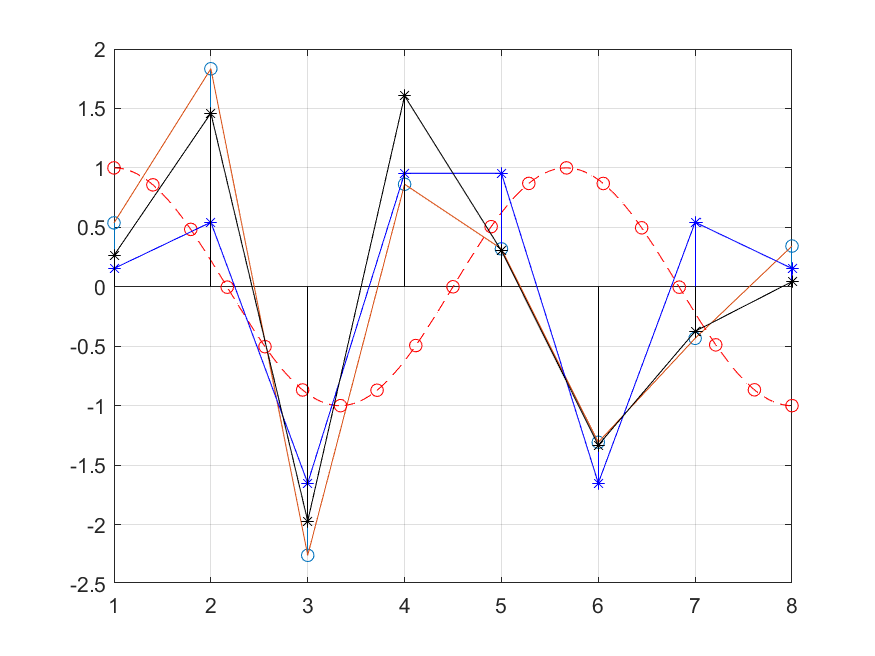
\includegraphics[width=0.8\textwidth]{Figure_1.png}
  \label{fig:music}
\end{figure}
\subsection{Signal Compression}

\section{Results}


Relative error for each compressed signal.
\begin{verbatim}
Relative error for x8: 0.000000
Relative error for x4: 0.285065
Relative error for x2: 0.564616
\end{verbatim}
What numerical results were obtained?
What do they represent?
Briefly summarize this section.

\section{Summary and Conclusion}
For this project, I first load the signal as a matrix file; then use matlab to compress the matrix to different extent using largest value method, use x2 to represent the matrix with 6 compressed signal in each column vector and x4 to represent the matrix with 4 compressed signal in each column vector; finally, calculate the relative error relative to the original matrix x. \\
According to the final result of relative error, the more the signal is compressed, the less like the sound to the original, which is represented using relative error. From the result part, the relative error of x2 is 0.56; that of x4 is 0.29; and that of x8 is 0. X2 has only 25 percent in each column vector that were not compressed, and x4 has 50 percent in each column vector that were not compressed, while x8 restore the original signal. So no double that relative error of x8 will be nearly 0. Because x4 has twice as much as that of x2 whose signal is not compressed. The relative error is nearly half as that of x2, as my expected.  


\section{References}
What I did for chatgpt:
For part g, the whole question, I asked the chatgpt because I don't know what the function to write using matlab.\\
Here is the list of functions:\\
1, finding absolute value-abs();\\
2, finding largest two values-maxk(, 2);\\
3, assign a to a2-a2(indices) = a(indices);\\
I also ask about some latex grammar:\\
Using textt to write the file name\\
how to insert a equation in the report\\
\end{document}
